\subsection{Space Confinement}

Since our drone could potentially move in unexpected ways whilst dancing, we confined it to move only in an allowable volume of space. This space is defined vertically by an altitude limit, and horizontally by an area marked by roundels on the ground.\\

\subsubsection{Vertical Limit}

We have two measures for imposing an altitude limit. The first is an ``absolute" limit where we manually configure the drone's internal altitude limit to 3.5m above the ground. Should the drone reach this altitude, the drone will automatically stop moving, land, and end the program, thus preventing the drone from flying into the ceiling. Realistically, we don't want the drone to stop and land in the middle of a dance routine, so we implemented a second ``soft" limit where we continually track altitude by receiving and reading the drone's navigation data, and if the drone reaches an altitude of 2.5m, our program will instruct the drone to move down for a short duration (2s). The drone will then continue to dance from where it should now be in the routine, after accounting for the 2s delay when the drone was moving down.\\

\textcolor{red}{make sure code reflects these values: altitude limit = 3500, soft limit = 2500, move down duration = 2s}\\

\subsubsection{Horizontal Limit}

For the horizontal limit, we first laid out a number of roundels on the floor to mark the area above which the drone may fly.

\begin{figure}[H]
      \centering
      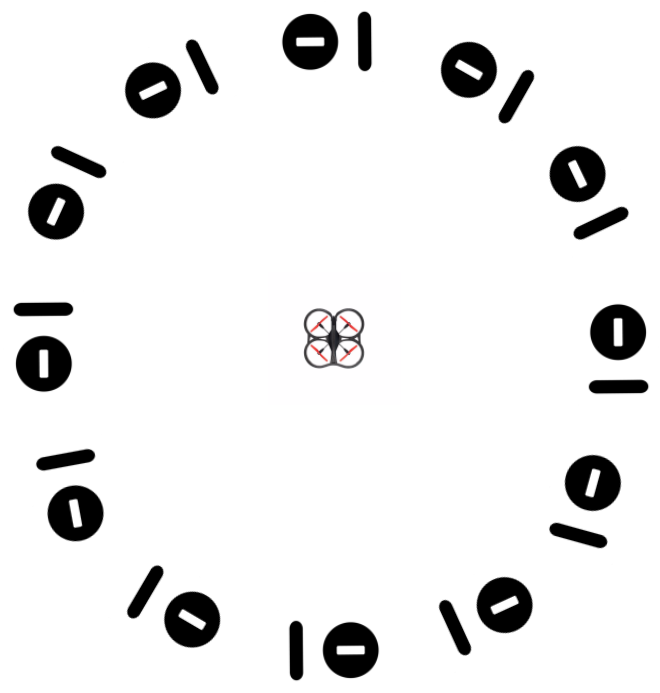
\includegraphics[width=0.8\linewidth]{3d-roundels-arranged.png}
      \caption{Bird's-eye view example of an area marked by roundels on the ground}
\end{figure}

We then configured the drone to use the ground-facing camera so that it can detect the roundel targets. When a roundel target is detected, the program will take the drone's relative orientation then calculate the necessary x- and y-directions for the drone to move away from the roundel without rotation. For example, in Figure \ref{fig:3d-angles} below, the blue vector indicates the current velocity of the drone, and is measured against the positive x-axis of the roundel to product an orientation. Then, a transfer equation is applied to the orientation angle to obtain the x- and y-magnitudes of the desired velocity of the drone, which is labelled as the green vector.

\begin{figure}[H]
      \centering
      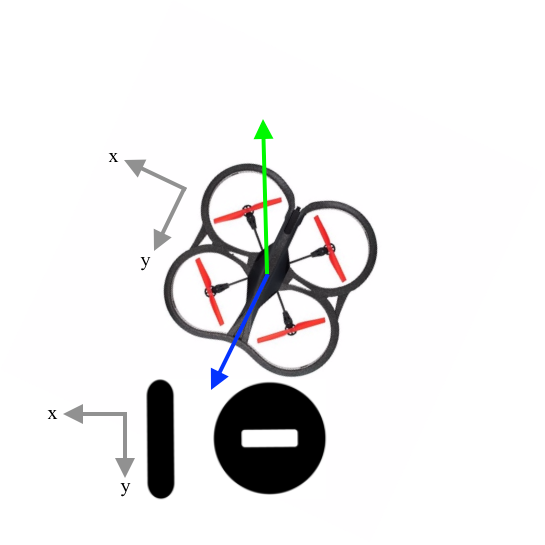
\includegraphics[width=1\linewidth]{3d-angles.png}
      \caption{\textit{blue} = current velocity, \textit{green} = desired velocity}
      \label{fig:3d-angles}
\end{figure}

The transfer functions required to convert orientation angle $\alpha$ into desired x-velocity $x$ and desired y-velocity $y$ with scaling factor $k$ are:

\begin{equation}
	x = k\times \cos(\alpha - \frac{\pi}{2})
\end{equation}

\begin{equation}
	y = k\times \sin(\alpha - \frac{\pi}{2})
\end{equation}

The ground camera of the AR Drone 2.0 has a 90� field of view. Combined with a maximum width of around around 80cm end-to-end between two roundels, the drone will need to be above at least 40cm above the ground to detect at least one roundel. Otherwise, there is a possibility that the drone slips between the gap between two roundels.

\begin{figure}[H]
      \centering
      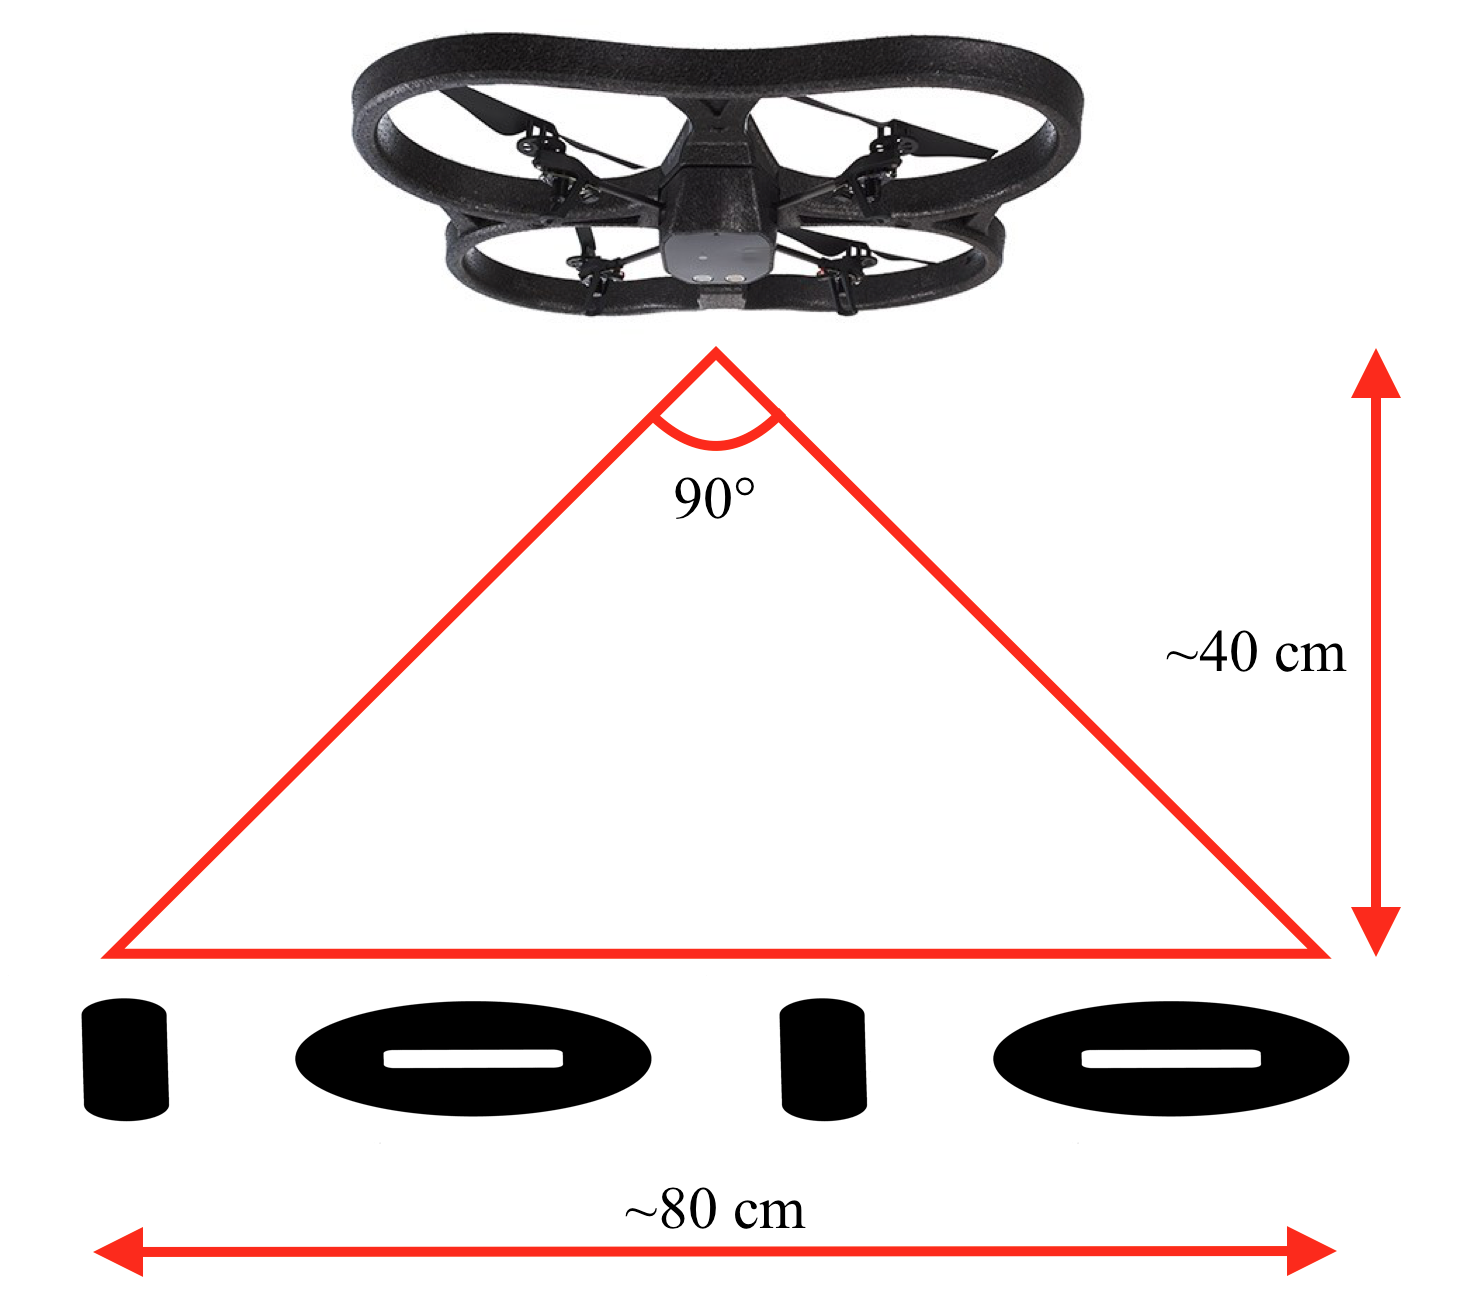
\includegraphics[width=0.8\linewidth]{3d-drone-fov.png}
      \caption{Field of view roundel detection requirement}
\end{figure}